
%(BEGIN_QUESTION)
% Copyright 2014, Tony R. Kuphaldt, released under the Creative Commons Attribution License (v 1.0)
% This means you may do almost anything with this work of mine, so long as you give me proper credit

I dette systemet gir et par differensialstrømsreléer (87) vern for en kraftlinje. Hvert relé måler strøm i alle tre faselederne i hver ende av linjen. Skråstreken og notasjonen ``$I_A$, $I_B$, $I_C$'' understreker at reléene overvåker alle tre faser:

$$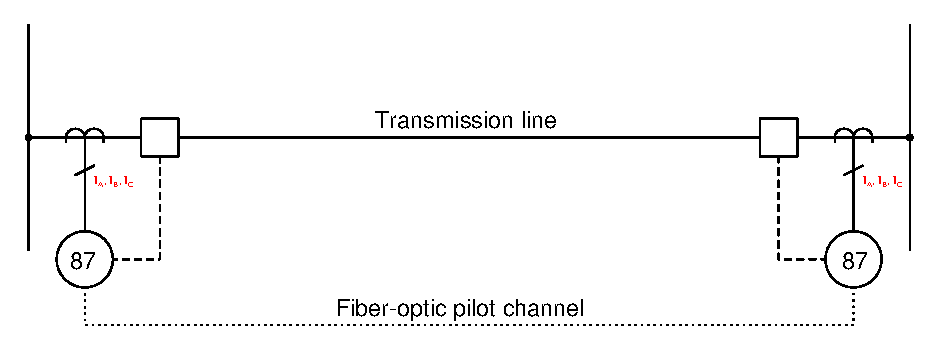
\includegraphics[width=15.5cm]{i00852x01.eps}$$

Anta at det oppstår en fase-til-fase-feil mellom fase A og B i kraftlinjen, uten noen forbindelse til jord. Avgjør om 87-reléene vil løse ut, og forklar hvorfor.

\underbar{file i00852}
%(END_QUESTION)





%(BEGIN_ANSWER)

En feil mellom fase A og B vil føre til at strøm forgrener seg fra begge lederne i feilpunktet. Dette skaper strømubalanse mellom endene (CT-målepunktene) i både fase A og fase B, og reléene detekterer differensialstrøm i linjen.

\vskip 10pt

Et øyeblikksbilde av strømmer viser avviket i begge faser:

$$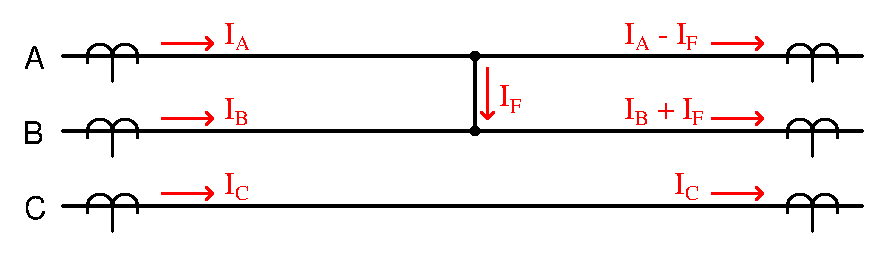
\includegraphics[width=15.5cm]{i00852x02.eps}$$

Ved en ikke-triviell feilstrøm $I_F$ er strømmen i hver ende av fase A tydelig ulik ($I_A \neq I_A - I_F$). Tilsvarende for fase B: ($I_B \neq I_B + I_F$). Dermed kan de to 87-reléene, som sammenligner fase-strømmer i begge ender av kraftlinjen, fastslå at det finnes en fasefeil et sted mellom CT-settene.

%(END_ANSWER)





%(BEGIN_NOTES)


%INDEX% Protective relay: differential current (87)

%(END_NOTES)
